\documentclass{article}[11pt]

\usepackage{amsmath}
\usepackage{amssymb}
\usepackage{nicefrac}

\usepackage{pdflscape}

\usepackage{upgreek}

\usepackage{bashful}

% No intendation
\setlength\parindent{0pt}

\usepackage{hyperref}

\usepackage{siunitx}
\sisetup{
  per-mode=fraction,
  fraction-function=\tfrac
}

\usepackage{listings}
  \lstset{
    basicstyle=\ttfamily,
    escapeinside=||,
    xleftmargin=1cm
  }

\usepackage{float}

\usepackage{longtable}

\usepackage{multirow}

\usepackage{tikz}
  \usetikzlibrary{patterns}
  \usetikzlibrary{arrows.meta}
  \usetikzlibrary{shapes.misc}
  \usetikzlibrary{calc}

\usepackage{pgfplots}

\usepackage{cleveref}
\crefmultiformat{equation}{(#2#1#3)}{ and~(#2#1#3)}{, (#2#1#3)}{ and~(#2#1#3)}


\usepackage{acronym}
\usepackage[acronym,nonumberlist]{glossaries}
\glsdisablehyper
\makeglossaries
\newacronym{spice}{SPICE}{Simulation Program with Integrated Circuit Emphasis}
\newacronym{lef}{LEF}{Library Exchange Format}
\newacronym{dft}{DFT}{Discrete Fourier Transform}
\newacronym{dtft}{DTFT}{Discrete-Time Fourier Transform}
\newacronym{fft}{FFT}{Fast Fourier Transform}
\newacronym{mosfet}{MOSFET}{Metal–Oxide–Semiconductor Field-Effect Transistor}
\newacronym{clm}{CLM}{Channel Length Modulation}
\newacronym{de}{DE}{differential equation}
\newacronym{soi}{SOI}{silicon-on-insulator}
\newacronym{ldo}{LDO}{low-dropout regulator}
\newacronym{ota}{OTA}{operational-transconductance amplifier}
\newacronym{ofa}{OFA}{operational-floating amplifier}

% literature
\usepackage[ backend=biber
           , isbn=true
           , sorting=none
           , style=ieee
           ]{biblatex}
\addbibresource{./../../literature.bib}

% definitions
\def \whatis       {Notes}
\def \title        {Fuubar}

\def \author       {Matthias Schweikardt}

\def \authorMail   {mschweikardt@posteo.de}

\def \authorGithub {mschweikardt}

\def \license      {CC BY-SA 4.0}
\def \licenseUrl   {https://creativecommons.org/licenses/by-sa/4.0/}

\def \date         {nodate}

\def \pdfurl       {https://mschweikardt.github.io/ee-notes/%
\bash[stdout]
IFS=/ 
var=($PWD)
echo ${var[-1]}
\END%
.pdf
}
\def \srcurl       {srcurl}


% Customize footer and header of document
\usepackage{fancyhdr}

% Access last page number
\usepackage{lastpage}

% Access last page number
\usepackage[thinc]{esdiff}

% Physics
\usepackage{physics}

% Comment environment
\usepackage{comment}

% Subcaptions
\usepackage{subcaption}

% Thicker lines in tables
\usepackage{booktabs}

% Indentation in footnote
\makeatletter
\renewcommand\@makefntext[1]{\leftskip=2em\hskip-0.5em\@makefnmark#1}
\makeatother         

% qty with the siunitx definition
\AtBeginDocument{\RenewCommandCopy\qty\SI}

% TikZ compatibility
\pgfplotsset{compat=1.18}


\makeatletter
\pgfmathdeclarefunction{myatan2}{2}{%
\begingroup%
  \pgfmathfloattofixed{#1}\edef\tempa{\pgfmathresult}%
  \pgfmathfloattofixed{#2}%
  \pgfkeys{pgf/fpu=false}%
  \pgfmathparse{atan2(\tempa,\pgfmathresult)}\pgfkeys{/pgf/fpu}%
  \pgfmathfloatparsenumber{\pgfmathresult}%
  \pgfmath@smuggleone\pgfmathresult%
\endgroup
}
\makeatother

\usepackage{tabularx}
% usepackages
\usepackage[ a4paper
           , textwidth  = 16.0cm
           , textheight = 25.0cm
           , headsep    =  0.25cm
           , voffset    =  0.3cm
           , footskip   =  1.25cm
           ]{geometry}

% Section and subsection enumeration
\renewcommand{\thesection}{\Roman{section}.} 
\renewcommand{\thesubsection}{\thesection\Alph{subsection}}

\usepackage{titlesec}
\titleformat{\section}
  {\normalfont\Large\bfseries}{\thesection}{0.2em}{}
\titleformat{\subsection}
  {\normalfont\large\bfseries}{\thesubsection}{0.2em}{}


% Defince title of document
\newcommand{\notetitle}{
  \begingroup
  \hypersetup{hidelinks}
  \thispagestyle{notefirst}
  \begin{center}
  \rule{\textwidth}{1pt}\\
  \medskip
  {\it \whatis}\\
  \bigskip
  {\LARGE \textbf{\title}}\\
  \medskip
  {\small \author}\\
  \rule{\textwidth}{0.5pt}\\
  {\small
    \begin{minipage}[t]{0.5\textwidth}
      \begin{tabular}[t]{ p{2.25cm} p{5.75cm}}
        Mail: & \href{mailto:\authorMail}{\tt{\authorMail}} \\
        Github: & \href{https://github.com/\authorGithub}{\tt{\authorGithub}} \\
      \end{tabular}
    \end{minipage}%
    %
    \begin{minipage}[t]{0.5\textwidth}
      \begin{tabular}[t]{ p{2.25cm} p{5.75cm} }
        Date: & \date  \\
        License: & \href{\licenseUrl}{\license}
      \end{tabular}
    \end{minipage}
  }%
  {\small
    \begin{minipage}[t]{\textwidth}
      \begin{tabular}[t]{ p{2.25cm} p{12cm}}
        Latest PDF: & \href{\pdfurl}{\tt{\pdfurl}} \\
        Latest Source: & \href{\srcurl}{\tt{\srcurl}}
      \end{tabular}
    \end{minipage}%
  }
  \bigskip
  \rule{\textwidth}{1pt}
  \end{center}
  \endgroup
}

% Header and footer on first page
\fancypagestyle{notefirst}{
  \fancyhf{}
  \renewcommand{\headrulewidth}{0pt}
  \renewcommand{\footrulewidth}{0pt}

  \fancyfoot[C]{\thepage/\pageref*{LastPage}}
}

% Header and footer on 2nd-last page
\fancypagestyle{noterest}{
  \fancyhf{}
  \renewcommand{\headrulewidth}{0.5pt}
  \renewcommand{\footrulewidth}{0.0pt}

  \fancyhead[L]{\author}
  \fancyhead[C]{\title}
  \fancyhead[R]{\date}

  \fancyfoot[C]{\thepage/\pageref*{LastPage}}
}
\pagestyle{noterest}

\usepackage{amsmath}
\usepackage{amssymb}
\usepackage{nicefrac}

\usepackage{pdflscape}

\usepackage{upgreek}

\usepackage{bashful}

% No intendation
\setlength\parindent{0pt}

\usepackage{hyperref}

\usepackage{siunitx}
\sisetup{
  per-mode=fraction,
  fraction-function=\tfrac
}

\usepackage{listings}
  \lstset{
    basicstyle=\ttfamily,
    escapeinside=||,
    xleftmargin=1cm
  }

\usepackage{float}

\usepackage{longtable}

\usepackage{multirow}

\usepackage{tikz}
  \usetikzlibrary{patterns}
  \usetikzlibrary{arrows.meta}
  \usetikzlibrary{shapes.misc}
  \usetikzlibrary{calc}

\usepackage{pgfplots}

\usepackage{cleveref}
\crefmultiformat{equation}{(#2#1#3)}{ and~(#2#1#3)}{, (#2#1#3)}{ and~(#2#1#3)}


\usepackage{acronym}
\usepackage[acronym,nonumberlist]{glossaries}
\glsdisablehyper
\makeglossaries
\newacronym{spice}{SPICE}{Simulation Program with Integrated Circuit Emphasis}
\newacronym{lef}{LEF}{Library Exchange Format}
\newacronym{dft}{DFT}{Discrete Fourier Transform}
\newacronym{dtft}{DTFT}{Discrete-Time Fourier Transform}
\newacronym{fft}{FFT}{Fast Fourier Transform}
\newacronym{mosfet}{MOSFET}{Metal–Oxide–Semiconductor Field-Effect Transistor}
\newacronym{clm}{CLM}{Channel Length Modulation}
\newacronym{de}{DE}{differential equation}
\newacronym{soi}{SOI}{silicon-on-insulator}
\newacronym{ldo}{LDO}{low-dropout regulator}
\newacronym{ota}{OTA}{operational-transconductance amplifier}
\newacronym{ofa}{OFA}{operational-floating amplifier}

% literature
\usepackage[ backend=biber
           , isbn=true
           , sorting=none
           , style=ieee
           ]{biblatex}
\addbibresource{./../../literature.bib}

% definitions
\def \whatis       {Notes}
\def \title        {Fuubar}

\def \author       {Matthias Schweikardt}

\def \authorMail   {mschweikardt@posteo.de}

\def \authorGithub {mschweikardt}

\def \license      {CC BY-SA 4.0}
\def \licenseUrl   {https://creativecommons.org/licenses/by-sa/4.0/}

\def \date         {nodate}

\def \pdfurl       {https://mschweikardt.github.io/ee-notes/%
\bash[stdout]
IFS=/ 
var=($PWD)
echo ${var[-1]}
\END%
.pdf
}
\def \srcurl       {srcurl}


% Customize footer and header of document
\usepackage{fancyhdr}

% Access last page number
\usepackage{lastpage}

% Access last page number
\usepackage[thinc]{esdiff}

% Physics
\usepackage{physics}

% Comment environment
\usepackage{comment}

% Subcaptions
\usepackage{subcaption}

% Thicker lines in tables
\usepackage{booktabs}

% Indentation in footnote
\makeatletter
\renewcommand\@makefntext[1]{\leftskip=2em\hskip-0.5em\@makefnmark#1}
\makeatother         

% qty with the siunitx definition
\AtBeginDocument{\RenewCommandCopy\qty\SI}

% TikZ compatibility
\pgfplotsset{compat=1.18}


\makeatletter
\pgfmathdeclarefunction{myatan2}{2}{%
\begingroup%
  \pgfmathfloattofixed{#1}\edef\tempa{\pgfmathresult}%
  \pgfmathfloattofixed{#2}%
  \pgfkeys{pgf/fpu=false}%
  \pgfmathparse{atan2(\tempa,\pgfmathresult)}\pgfkeys{/pgf/fpu}%
  \pgfmathfloatparsenumber{\pgfmathresult}%
  \pgfmath@smuggleone\pgfmathresult%
\endgroup
}
\makeatother

\usepackage{tabularx}


\def \title  {CMOS Schmitt-Trigger}
\def \date   {May 30, 2025}

\def \pdfurl {https://mschweikardt.github.io/ee-notes/cmos-schmitt-trigger.pdf}
\def \srcurl {https://github.com/mschweikardt/ee-notes/tree/main/notes/cmos-schmitt-trigger}

\usepackage[scale=5]{draftwatermark}

\begin{document}

\notetitle

\cite{wang-schmitttrigger-91,filanovsky-schmitttrigger-94,melek-schmitttrigger-17}

Fig. \ref{fig:schmitt-trigger} shows the schematic of a CMOS Schmitt-Trigger
and Fig. \ref{fig:vtc} the Voltage Transfer Characteristic (VTC).

\begin{figure}[H]
  \centering
  \begin{circuitikz}
    \input{./../../tikzlib/figs/cmos-schmitt-trigger-schematic-a.tex}
  \end{circuitikz}
  \caption{Schematic of the Schmitt-Trigger}
  \label{fig:schmitt-trigger}
\end{figure}

\begin{figure}[H]
  \centering
  \begin{tikzpicture}
    \input{./../../tikzlib/figs/cmos-schmitt-trigger-transfer-char-a.tex}
  \end{tikzpicture}
  \caption{Voltage Transfer Characteristic of the Schmitt-Trigger}
  \label{fig:vtc}
\end{figure}

We have to investigate the NMOS Branch
(\texttt{NM0}, \texttt{NM1} and \texttt{NM2}) for deriving $V_{\mathrm{I,p}}$
and the PMOS Branch (\texttt{PM0}, \texttt{PM1} and \texttt{PM2})
for deriving $V_{\mathrm{I,n}}$.
We will observe the point where the transistor \texttt{NM1} is starting to
conduct, i.e.
\begin{equation}\label{eq:cond-sw-vip}
 V_{\mathrm{GS1N}} = V_{\mathrm{TN1}}
\end{equation}
or
\begin{equation}
  V_{\mathrm{X}} = V_{\mathrm{I,p}} - V_{\mathrm{TN1}}.
\end{equation}
The modes of the transistors for \eqref{eq:cond-sw-vip} are shown in 
Tab.~\ref{tab:mode-nmos-branch}.
\begin{table}[H]
  \centering
  \caption{Mode of the transistors in the NMOS-Branch at the
           switching threshold $V_{\mathrm{I,p}}$}
  \begin{tabular}{|c|c|c|c|}
                                                                                                                                                             \hline
    Device       & $V_{\mathrm{GS}}$                                   & $V_{\mathrm{DS}}$                                     & Mode                     \\ \hline \hline
    \texttt{NM0} & $V_{\mathrm{I,p}}$                                  & $V_{\mathrm{I,p}} - V_{\mathrm{TN1}}$                 & ohmic \footnotemark      \\ \hline
    \texttt{NM1} & $V_{\mathrm{TN1}}$                                  & $V_{\mathrm{DD}}-V_{\mathrm{I,p}}+V_{\mathrm{TN1}}$   & off \footnotemark        \\ \hline   
    \texttt{NM2} & $V_{\mathrm{DD}}-V_{\mathrm{I,p}}+V_{\mathrm{TN1}}$ & $V_{\mathrm{DD}} - V_{\mathrm{I,p}}+V_{\mathrm{TN1}}$ & saturation \footnotemark \\ \hline   
  \end{tabular}
  \label{tab:mode-nmos-branch}
\end{table}
\footnotetext[1]{
  $V_{\mathrm{GS0}}=V_{\mathrm{I,p}}>V_{\mathrm{TN0}}$, 
  $V_{\mathrm{GS0}}-V_{\mathrm{TN0}}=V_{\mathrm{I,p}}-V_{\mathrm{TN0}}>
   V_{\mathrm{DS,0}}=V_{\mathrm{I,p}} - V_{\mathrm{TN1}}$ , because
  $V_{\mathrm{TN0}}<V_{\mathrm{TN1}}$
 }
\footnotetext[2]{
  $V_{\mathrm{GS1N}}=V_{\mathrm{I,p}}-V_{\mathrm{X}}=V_{\mathrm{TN1}} \leq V_{\mathrm{TN1}}$
 }
\footnotetext[3]{
  $V_{\mathrm{GS2N}}=V_{\mathrm{DD}} - V_{\mathrm{I,p}}+V_{\mathrm{TN1}}>
   V_{\mathrm{TN2}}$,
   $V_{\mathrm{GS2N}}-V_{\mathrm{TN2}}=
    V_{\mathrm{DD}}-V_{\mathrm{I,p}}+V_{\mathrm{TN1}}-V_{\mathrm{TN2}}<
    V_{\mathrm{DS2NN}}=V_{\mathrm{DD}} - V_{\mathrm{I,p}}+V_{\mathrm{TN1}}$
 }
By applying KCL at node \texttt{X} we get
\begin{equation}\label{eq:kcl-x}
 \underbrace{I_{\mathrm{D1}}}_{=0} + I_{\mathrm{D2}} = I_{\mathrm{D0}}.
\end{equation}
From the transistor equations and Tab.~\ref{tab:mode-nmos-branch} we get
\begin{align}\label{eq:id0}
 I_{\mathrm{D0}} 
 & = \mu_0 C_{\mathrm{Ox}} \frac{w_{\mathrm{N0}}}{l_{\mathrm{N0}}}
     \left[\left(V_{\mathrm{GS0}}-V_{\mathrm{TN0}}\right)V_{\mathrm{DS0}}
           -\frac{1}{2}V_{\mathrm{DS0}}^2\right] \nonumber \\
 & = \mu_0 C_{\mathrm{Ox}} \frac{w_{\mathrm{N0}}}{l_{\mathrm{N0}}}
     \left[\left(V_{\mathrm{I,p}}-V_{\mathrm{TN0}}\right)\left(V_{\mathrm{I,p}}
           - V_{\mathrm{TN1}}\right)-\frac{1}{2}\left(V_{\mathrm{I,p}} 
           - V_{\mathrm{TN1}}\right)^2\right]
\end{align}
and
\begin{align}\label{eq:id2}
 I_{\mathrm{D2}} 
  & = \frac{1}{2} \mu_0 C_{\mathrm{Ox}} \frac{w_{\mathrm{N2}}}{l_{\mathrm{N2}}}
      \left(V_{\mathrm{GS2N}}-V_{\mathrm{TN2}}\right)^2 \nonumber \\
  & = \frac{1}{2} \mu_0 C_{\mathrm{Ox}} \frac{w_{\mathrm{N2}}}{l_{\mathrm{N2}}}
      \left(V_{\mathrm{DD}} - V_{\mathrm{I,p}}
            +V_{\mathrm{TN1}}-V_{\mathrm{TN2}}\right)^2
\end{align}

Using \eqref{eq:kcl-x}, \eqref{eq:id0}, \eqref{eq:id2} and
$V_{\mathrm{TN0}} \approx V_{\mathrm{TN1}} \approx
 V_{\mathrm{TN2}} \approx V_{\mathrm{TN}}$
we get
\begin{equation}\label{eq:vip}
 V_{\mathrm{I,p}} = 
 \frac{V_{\mathrm{DD}}+\sqrt{\frac{w_{\mathrm{N0}}}{w_{\mathrm{N3}}}}V_{\mathrm{TN}}}
      {1+\sqrt{\frac{w_{\mathrm{N0}}}{w_{\mathrm{N3}}}}}.
\end{equation}
The function~\eqref{eq:vip} is shown in Fig.~\ref{fig:vip}.
\begin{figure}[H]
  \centering
  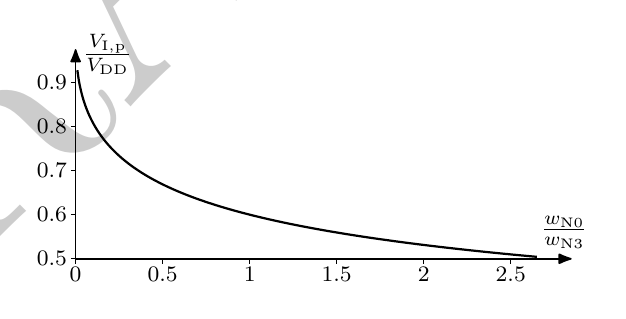
\begin{tikzpicture}[]
    \begin{axis}[ xmin=0
                , xmax=2.85,
                , ymin=0.5
                , ymax=0.975,
                , xtick={0.5,1.0,1.5,2.0,2.5}
                , ytick={0.6,0.7,0.8,0.9}
                , extra x ticks={0}
                , extra x tick labels={0}
                , extra y ticks={0.5}
                , extra y tick labels={0.5}
                , inner axis line style={semithick,black}
                , axis lines=center
                , axis line style={-Latex[round]}
                , every axis x label/.style={ at={(ticklabel* cs:0.985)}
                                            , anchor=south
                                            , inner sep=3.5pt
                                            }
                , every axis y label/.style={ at={(ticklabel* cs:0.975)}
                                            , anchor=west
                                            , inner sep=2.5pt
                                            }
                , clip=false
                , major tick length=1.75pt
                , xlabel=$\frac{w_{\mathrm{N0}}}{w_{\mathrm{N3}}}$
                , ylabel= $\frac{V_{\mathrm{I,p}}}{V_{\mathrm{DD}}}$
                , width=0.65\textwidth
                , height=0.35\textwidth
                , yticklabel style = {font=\footnotesize,xshift=0.5ex}
                , xticklabel style = {font=\footnotesize,yshift=0.5ex}
                , every tick/.style={black}
                , tick align=outside
                ]
    \addplot[ mark=none
        , very thick
        , domain=0.01:2.65
        , samples=300
        , smooth
        , thick] {(1+sqrt{\x}*0.2)/(1+sqrt{\x})};   
    \end{axis}
  \end{tikzpicture}
  \caption{Threshold $V_{\mathrm{I,p}}$ for
           $V_{\mathrm{TN}}=0.2 \cdot V_{\mathrm{DD}}$}
  \label{fig:vip}
\end{figure}

\printbibliography
\end{document}